\documentclass[12pt,a4paper, reqno]{amsart}
% ukazi za delo s slovenscino -- izberi kodiranje, ki ti ustreza
\usepackage[slovene]{babel}
%\usepackage[cp1250]{inputenc}
%\usepackage[T1]{fontenc}
\usepackage[utf8]{inputenc}
\usepackage{amsmath,amssymb,amsfonts}
\usepackage{url}
%\usepackage[normalem]{ulem}
\usepackage[dvipsnames,usenames]{color}
\usepackage{eurosym}
\usepackage{graphicx}
\usepackage{adjustbox}



% ne spreminjaj podatkov, ki vplivajo na obliko strani
\textwidth 15cm
\textheight 24cm
\oddsidemargin.5cm
\evensidemargin.5cm
\topmargin-5mm
\addtolength{\footskip}{10pt}
\pagestyle{plain}
\overfullrule=15pt % oznaci predlogo vrstico


% ukazi za matematicna okolja
\theoremstyle{definition} % tekst napisan pokoncno
\newtheorem{definicija}{Definicija}[section]
\newtheorem{primer}[definicija]{Primer}
\newtheorem{opomba}[definicija]{Opomba}

\renewcommand\endprimer{\hfill$\diamondsuit$}


\theoremstyle{plain} % tekst napisan posevno
\newtheorem{lema}[definicija]{Lema}
\newtheorem{izrek}[definicija]{Izrek}
\newtheorem{trditev}[definicija]{Trditev}
\newtheorem{posledica}[definicija]{Posledica}


% za stevilske mnozice uporabi naslednje simbole
\newcommand{\R}{\mathbb R}
\newcommand{\N}{\mathbb N}
\newcommand{\Z}{\mathbb Z}
\newcommand{\C}{\mathbb C}
\newcommand{\Q}{\mathbb Q}


% ukaz za slovarsko geslo
\newlength{\odstavek}
\setlength{\odstavek}{\parindent}
\newcommand{\geslo}[2]{\noindent\textbf{#1}\hspace*{3mm}\hangindent=\parindent\hangafter=1 #2}


% naslednje ukaze ustrezno popravi
\newcommand{\program}{Finančna matematika} % ime studijskega programa: Matematika/Finančna matematika
\newcommand{\imeavtorja}{Žan Jarc} % ime avtorja
\newcommand{\imementorja}{izr.~prof.~dr. Damjana Kokol Bukovšek} % akademski naziv in ime mentorja
\newcommand{\imesomentorja}{asist.~dr. Aleš Toman}
\newcommand{\naslovdela}{Finančni instrumenti osnovani na razpršenosti}
\newcommand{\letnica}{2021} %letnica diplome


% vstavi svoje definicije ...




\begin{document}

% od tod do povzetka ne spreminjaj nicesar
\thispagestyle{empty}
\noindent{\large
UNIVERZA V LJUBLJANI\\[1mm]
FAKULTETA ZA MATEMATIKO IN FIZIKO\\[5mm]
\program\ -- 1.~stopnja}
\vfill

\begin{center}{\large
\imeavtorja\\[2mm]
{\bf \naslovdela}\\[10mm]
Delo diplomskega seminarja\\[1cm]
Mentorica: \imementorja \\[0.3cm]
Somentor: \imesomentorja}

\end{center}
\vfill

\noindent{\large
Ljubljana, \letnica}
\pagebreak

\thispagestyle{empty}
\tableofcontents
\pagebreak

\thispagestyle{empty}
\begin{center}
{\bf \naslovdela}\\[3mm]
{\sc Povzetek}
\end{center}
% tekst povzetka v slovenscini
V povzetku na kratko opiši vsebinske rezultate dela. Sem ne sodi razlaga organizacije dela -- v katerem poglavju/razdelku je kaj, pač pa le opis vsebine.
\vfill
\begin{center}
{\bf Angleški naslov dela}\\[3mm] % prevod slovenskega naslova dela
{\sc Abstract}
\end{center}
% tekst povzetka v anglescini
Prevod zgornjega povzetka v angleščino.

\vfill\noindent
{\bf Math. Subj. Class. (2020):} navedi vsaj eno klasifikacijsko oznako -- dostopne so na \url{www.ams.org/mathscinet/msc/msc2020.html}  \\[1mm]
{\bf Ključne besede:} navedi nekaj ključnih pojmov, ki nastopajo v delu  \\[1mm]
{\bf Keywords:} angleški prevod ključnih besed
\pagebreak



% tu se zacne besedilo seminarja
\section{Uvod}
Finančni trg sestavljajo vrednostni papirji, katerih vrednosti se v času spreminjajo. Zaradi spreminjanja vrednosti vsak vrednostni papir ali pa portfelj papirjev ustvarja donose ali izgube. Če donos ali izgubo delimo z začetno vrednostjo papirja ali portfelja, temu rečemo donostnost, ki je izražena v odstotkih in je lahko pozitivna ali negativna. Razpršenost donosnosti v časovnem obdobju z določeno dolžino je lahko večja ali manjša. Standardnemu odklonu porazdelitve donosnosti rečemo volatilnost vrednostnega papirja ali portfelja.\\

Investitorji lahko s pomočjo informacije o volatilnosti potencialne naložbe ugotovijo, kako tvegana je njihova investicija. Pri vlaganju v finančno naložbo z nizko volatilnostjo se pričakuje, da bo donosnost investicije morda nizka, vendar precej netvegana, medtem ko nam lahko investicija v finančno naložbo z visoko volatilnostjo prinese višjo donosnost, vendar tudi večje tveganje.\\

Finančni inštrumenti na osnovi volatilnosti so bili zasnovani z namenom, da vlagateljem ponudijo možnost, da trgujejo z razpršenostjo donosnosti in s tem zavarujejo svoj portfelj pred nenadnimi neugodnimi nihaji. V svojem delu diplomskega seminarja se bom posvetil indeksu volatilnosti (angl. \textit{volatiltiy index}) čikaške borze opcij (Chicago Board Option Exchange, CBOE), za katerega se pogosto uporablja tudi ime indeks VIX.
Indeks VIX je bil razvit za napovedovanje pričakovane volatilnosti in se izračunava s pomočjo podatkov o nakupnih in prodajnih opcijah na ameriški delniški indeks Standard \& Poor's 500.\\

V drugem poglavju bomo opisali indeks S\&P~500, kako ga izračunamo, prikazali njegovo gibanje skozi čas in opisali opcije na indeks. V tretjem poglavju bomo podobno naredili še za indeks VIX. V četrtem poglavju bomo analizirali gibanji obeh indeksov in opisali terminske pogodbe in opcije na indeks VIX, s katerimi se lahko vlagatelji zavarujejo pred padcem vrednosti indeksa S\&P~500.


\section{Indeks Standard \& Poor's 500}
Indeks Standard \& Poor's 500 ali indeks S\&P 500 je najpogosteje uporabljeni pokazatelj stanja v ameriškem gospodarstvu. Prva objava indeksa je bila 4. marca 1957 s strani družbe S\&P Dow Jones Indices. Pri izračunu indeksa uporabljajo podatke o 500 največjih ameriških podjetij, ki najbolj reprezentativno predstavljajo ameriški delniški trg. Če na primer v ameriškem delniškem trgu 20 odstotni delež predstavljajo industrijska podjetja, bo tudi skupna kapitalizacija v indeks vključenih industrijskih podjetij predstavljala 20 odstotkov celotne kapitalizacije indeksa.
Vrednosti indeksa se na borznih trgih pojavljajo pod kratico GSPC, SPX, ... 
Najbolj znana podjetja, ki so vključena v indeks S\&P 500 so \cite{spx_companies}:
\begin{itemize}
\item Apple (6,27~\% delež kapitalizacije v indeksu).\\

\item Alphabet (6,72~\%).\\

\item General Motors (0,16~\%).\\

\item Goldman Sachs (0,36~\%).\\
\end{itemize}


\subsection{Izračun vrednosti indeksa S\&P 500}
Indeks S\&P 500 je kapitalsko utežen. To pomeni, da spremembe vrednosti delnic podjetij z višjo tržno kapitalizacijo bolj vplivajo na spremembe vrednost indeksa kot spremembe vrednsti delnic podjetij z nižjo tržno kapitalizacijo. Kapitalsko uteženost opazimo tudi iz formule za izračun vrednosti $I_{500}$ indeka S\&P~500.
$$
I_{500} = \sum_{i=1}^{500}\frac{P_i \cdot{} Q_i}{D},
$$
kjer je:
\begin{itemize}
\item $P_i$ cena delnice $i$-tega podjetja.\\

\item $Q_i$ število za trgovanje razpoložljivih delnic $i$-tega podjeta.\\

\item $D$ indeksni delitelj (angl. \textit{index divisor}).\\
\end{itemize}

Pri izračunu indeksa uporabimo le tiste delnice, s katerimi se lahko prosto trguje, in ne kar celotne tržne kapitalizacije podjetja, saj se z določenim delom delnic podjeja ne more trgovati, ker so te namenjene za nagrajevanje zaposlenih. V primeru podjetja Apple je tržna kapitalizacija podjetja približno 2\,465 milijard dolarjev, medtem ko je bila prosta tržna kapitalizacija podjetja (angl. \textit{free-float market capitalization}) približno 2\,439 milijard dolarjev \cite{apple_capitalization}.\\
Indeksni delitelj $D$ pri izračunu vrednosti indeksa uporabljamo iz dveh razlogov:
\begin{itemize}
\item Če bi samo seštevali proste tržne kapitalizacije podjetij, bi dobili ogromno število, izraženo v dolarjih. Z deljenjem z indeksnim deliteljem dobimo manjše število brez enot.\\

\item Posamezno podjetje je lahko iz različnih razlogov odstranjeno iz indeksa in ga nadomesti primernejše podjetje. Indeksni delitelj poskrbi, da zaradi takih sprememb v sestavi indeksa ne prihaja do velikih sprememb v vrednosti indeksa, ki ne bi bile osnovane na resničnih spremembah na delniškem trgu.\\
\end{itemize}

Družba S\&P Dow Jones Indices ne razkriva, kako izračunavajo indeksni delitelj, vendar lahko podatek o vrednosti indeksnega delitelja izračunamo sami, če poznamo trenutno vrednost indeksa  S\&P~500 ter cene in število prostih delnic vseh 500 podjetij, ki sestavljajo indeks. Vrednost indeksnega delitelja junija 2021 je bila približno 8\,452 milijard dolarjev \cite{spx_devisor}.\\
\newpage
\subsection{Gibanje indeksa vrednosti S\&P 500 skozi čas}
Slika \ref{Graf 1} prikazuje vrednosti indeksa S\&P~500 v obdobju od leta 2004 do leta 2021. Na sliki lahko opazimo, da je vrednost indeksa, razen v redkih izjemah, rastla.
Opazimo samo tri večje padci; finančna kriza leta 2008, nenadni padec indeksa pozno leta 2018 in padec indeksa marca 2020 zaradi negotovosti ob izbruhu svetovne epidemije covida-19. \\

Medtem ko je bil padec leta 2018 kratkotrajen in se je vrednost indeksa vrnila nazaj na vrednosti pred padcem v nekaj mesecih, je finančna kriza leta 2008 pustila veliko dolgotrajnejše posledice, saj se je indeks vrnil na predkrizne vrednosti šele leta 2013, skoraj 5 let po zlomu finančnega sistema. \\

Čeprav je bil padec indeksa marca leta 2020 največji v zgodovini (vrednost indeksa S\&P~500 je iz do tedaj najvišje vrednosti 3\,380 padla za skoraj 33~\% na vrednost 2\,290), je bil le ta, podobno kot leta 2018, kratkotrajen. Indeks je nadoknadil izgubljeno vrednost v le 5 mesecih.  \\

Pregled gibanja vrednosti indeksa v zadnjih 17 letih nakazuje, da indeks S\&P~500 ni uporaben le za reprezentacijo ameriškega delinškega trga, ampak predstavlja dobro dolgoročno investicijo. Direktno v indeks ne moremo investirati, lahko pa izoblikujemo portfelj delnic, ki je po sestavi ekvivalenten sestavi indeksa. Ker pa je kupovanje delnic 500 podjetij drago in zamudno, na trgu obstajajo alternative; to so terminske pogodbe in opcije na vrednosti indeksa S\&P~500. V nadaljevanju si bomo pogledali samo opcije, saj so te ključne pri izračunu vrednosti indeksa VIX.
\begin{figure}[!h]
\centering
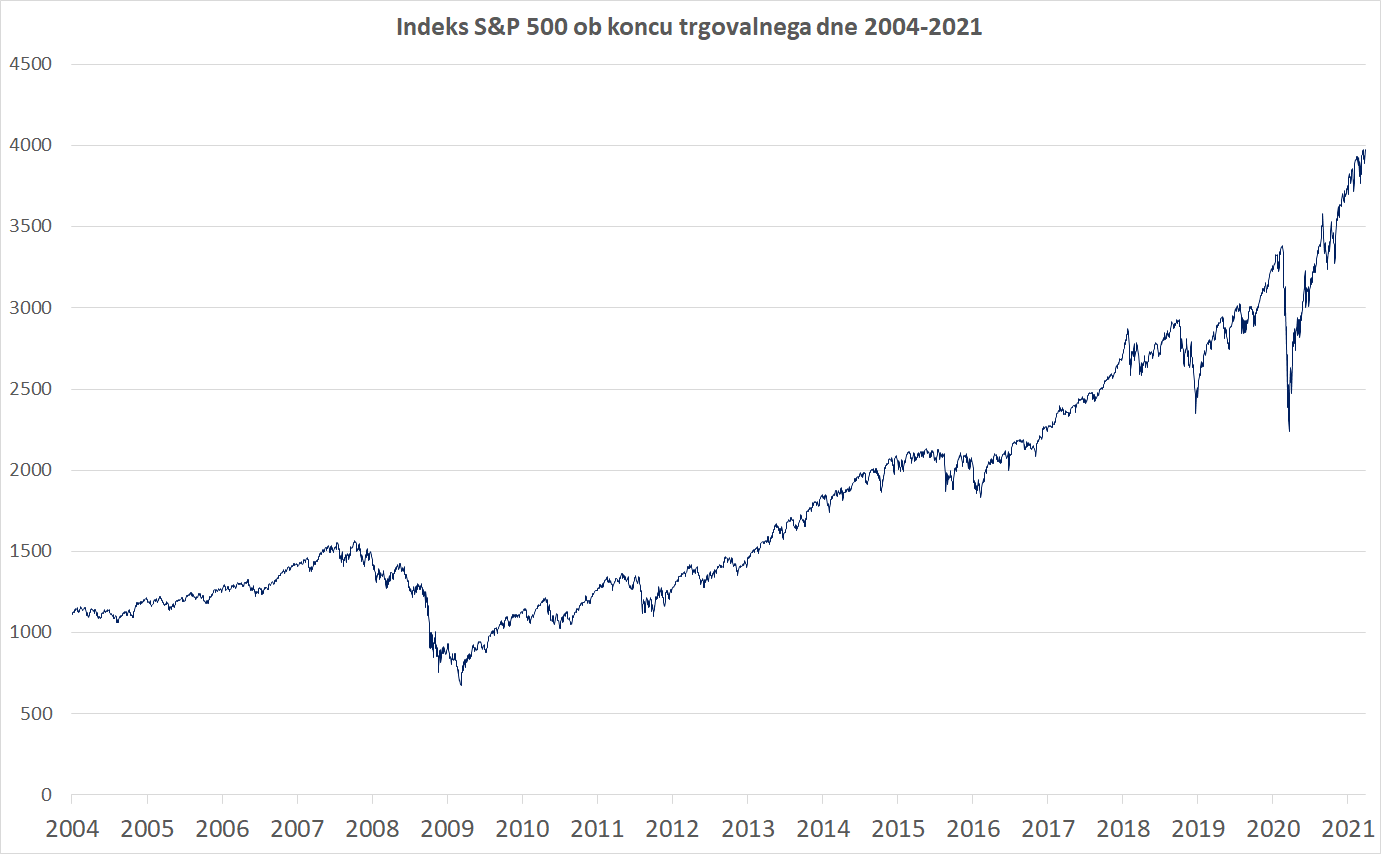
\includegraphics[width = 15 cm]{Grafi/SPX_2004-2021.png}
\caption{Gibanje vrednosti indeksa S\&P~500 v obdobju 2004--2021, vir: Yahoo finance}
\label{Graf 1}
\end{figure}


\subsection{Opcije na vrednost indeksa S\&P~500}

Indeks S\&P~500 s svojo vrednostjo zelo hitro odraža stanje na ameriškem delniškem trgu in je zato eden najbolj opazovanih delniških indeksov v finančnem svetu. Zaradi te popularnosti obstaja več tipov opcij na vrednost indeksa S\&P~500, ki se razlikujejo po oznaki, zapadlosti, uri poravnave in denarnem multiplikatorju. Tipi opcij, s katerimi lahko trgujemo na borzi CBOE so:
\begin{itemize}
\item Mesečne opcije na vrednost indeksa S\&P~500. Veljajo za tradicionalne opcije in jih najdemo pod oznako SPX. Mesečne opcije zapadejo na tretji petek v izbranem mesecu in se poravnajo na dan zapadlosti v dopoldanskih urah po vrednosti indeksa S\&P~500, ki je veljala ob začetku trgovanja. (angl. \textit{AM-settled}). Denarni multiplikator je 100 dolarjev.\\

\item Tedenske opcije (angl. \textit{Weeklys}) in opcije ob koncu meseca (angl. \textit{End of Month}). Medtem ko posamezne tedenske opcije zapadejo na ponedeljek, sredo ali petek v izbranem tednu in se poravnajo v popoldanskih urah po vrednosti indeksa S\&P~500 ob koncu trgovalnega dne (angl. \textit{PM-settled}), opcije ob koncu meseca zapadejo na zadnji delovni dan v izbranem mesecu in se prav tako poravnajo v popoldanskih urah. Obe vrsti opcij imata denarni multiplikator 100 dolarjev in oznako SPXW.\\

\item Mini S\&P~500 opcije (angl. \textit{Mini-SPX Index Options}), ki se prav tako delijo na tedenske opcije in opcije ob koncu meseca. Mini S\&P~500 opcije najdemo pod oznako XSP in imajo denarni multiplikator 10 dolarjev.\\
\end{itemize}

Vse naštete opcije so evropske in so, podobno kot večina indeksnih opcij, denarno poravnane.\\

\textbf{Zgled.} 
Oglejmo si primer nakupa in  poravnave mesečne nakupne opcije na vrednost indeksa S\&P~500.  Vrednost indeksa S\&P~500 na torek, 4. maja 2021, je bila 4\,164,66. Na ta dan smo želeli kupiti klasično mesečno nakupno opcijo na indeks S\&P~500 z zapadlostjo na tretji petek v avgustu, to je 20. avgusta 2021. Premija za avgustovsko nakupno opcijo z izvršilno vrednostjo 4\,250 je znašala  100,44.\
Zaradi denarnega multiplikatorja 100 dolarjev za nakup nakupne opcije plačamo
$$
100\, \$ \cdot 100,\!44 \, = 10\,044 \,\$.
$$
Če bi držali svojo pozicijo vse do zapadlosti opcije, bi se 20. avgusta 2021, opcija poravnala po vrednosti indeksa S\&P~500 ob koncu trgovalnega dne, ki je znašala 4\,412,14. Ker vrednost indeksa na trgu presega izvršilno vrednost, tem bi bilo naše izplačilo enako:
$$
(4\,412,\!14 - 4\,250) \cdot 100\,\$ = 16\,214\,\$,
$$
naš dobiček (če zanemarimo časovno vrednost denarja) pa:
$$
16\,214 \, \$ -10\,044 \, \$ = 6\,170\,\$.
$$


Strokovnjaki ocenjujejo, da je bila decembra 2020 skupna vrednost vseh izvedenih finančnih inštrumentov, odvisnih od vrednosti indeksa S\&P~500, enaka 13,5 bilijard dolarjev \cite{spx_cap}. Zaradi tako velike alokacije sredstev so za vlagatelje koristni finančni inštrumenti, ki bi jih obvarovali pred padcem vrednosti indeksa in posledično vseh investicij, odvisnih od vrednosti indeksa.


\section{Indeks volatilnosti}
Indeks volatilnosti čikaške borze opcij ali indeks VIX je bil razvit leta 1993 in se s spremenjeno metodologijo iz leta 2003 uporablja še danes. Indeks prikazuje 30-dnevno pričakovano volatilnost indeksa S\&P 500  in se izračuna s pomočjo nakupih in prodajnih opcij na indeks S\&P~500, ki se ne splačajo (angl. \textit{out-of-the-money}). Da lahko indeks res prikazuje 30-dnevno pričakovano volatilnost, za izračun njegove vrednosti uporabimo vse prej omenjene opcije, ki zapadejo čez več kot 23 in manj kot 37 dni. Za vsako zapadlost na borzi hkrati kotira več tipov opcij z različnimi izvršilnimi cenami. Za premijo posamezne opcije na borzi preberemo dve vrednosti:
\begin{itemize}
\item Ponujena premija (angl. \textit{bid}), ki je premija po kateri lahko posamezno opcijo kupimo.\\

\item Povprašana premija (angl. \textit{ask}), ki je permija po kateri lahko posamezno opcijo prodamo.\\
\end{itemize}
Povprečje povprašane in ponujene premije posamezne opcije je povprečna premija opcije.


\subsection{Izračun vrednosti indeksa VIX}
Kot že omenjeno, se pri izračunu vrednosti indeksa VIX upoštevajo vse nakupne in prodajne opcije na indeks S\&P 500, ki se ne splačajo in zapadejo čez več kot 23 dni in manj kot 37 dni.
Za vsako opcijo naprej določimo njen čas do zapadlosti $T$ izražen kot delež leta, določen na minuto natančno. Izračunamo ga po formuli:
$$
T = \frac{M_{\text{danasnji\, dan}} + M_{\text{dan\, poravnave}} + M_{\text{ostali\, dnevi}}} {\text{minute\, v\, letu}}
$$
kjer je:
\begin{itemize}
\item $M_{\text{danasnji\, dan}}$ preostalo število minut do polnoči današnjega dneva.\\

\item $M_{\text{dan\, poravnave}}$ je število minut od polnoči do 9:30 po vzhodnoameriškem času (angl. \textit{US East Coast Time}) za opcije na indeks S\&P~500, ki se poravnajo v dopoldanskih urah ali pa število minut od polnoči do 16:00  po vzhodnoameriškem času za opcije, ki se poravnajo v popoldanskih urah.\\

\item $ M_{\text{ostali\, dnevi}}$ pa je število minut preostalih dnevov do zapadlosti posamezne opcije.
\end{itemize}
Nato za vsak čas do zapadlosti $T$ iz krivulje donosnosti ameriških zakladnih obveznic določimo pripadajočo netvegano obrestno mero $R$.\\

Vse nakupne in prodajne opcije, ki zapadejo na isti dan, uredimo po velikosti izvršilne vrednosti $K_i$ in poiščemo tisti par nakupne in prodajne opcije z enako izvršilno vrednostjo, pri kateri je absolutna razlika $ |c_i - p_i|$ med povprečnima premija nakupne in prodajne opcije najmanjša. S tako dobljeno izvršilno vrednostjo $K$ in absolutno razliko $|c-p|$ med povprečnima premijama nakupne ter prodajne opcije nato izračunamo terminsko vrednost indeksa, določeno na osnovi premij indeksnih opcij (angl. \textit{forward index level derived from index option prices}), ki jo označimo z $F$ in dobimo po predpisu:
$$
F= K + e^{RT} \cdot (c-p).
$$
Nato za vsak dan zapadlosti opcij določimo najvišjo izvršilno vrednostjo $K_0$, ki je še manjša ali enaka od izračunane terminske vrednosti indeksa $F$ za tisti dan.\\

Pri izbiri prodajnih opcij, ki jih bomo uporablili za izračun indeksa VIX, so primerne le tiste z izvršilno vrednostjo manjšo ali enako $K_0$. Najprej izberemo tiste prodajne opcije, ki imajo izvršilno vrednost enako $K_0$. Nadaljujemo iskanje primernih prodajnih opcij z vse nižjo izvršilno vrednostjo, ki imajo ponujeno premijo večjo od 0. Ko se pri iskanju pojavita dve zaporedni opciji s ponujeno premijo enako nič, iskanje končamo in nobene prodajne opcije z nižjo izvršilno vrednostjo ne vključimo več v izračun vrednosti indeksa.\\

Podoben postopek opravimo tudi za iskanje primernih nakupnih opcij, le da pri tem iskanju upoštevamo le opcije z izvršilno vrednostjo večjo ali enako $K_0$. V izračun vključimo najprej tiste nakupne opcije, ki imajo izvršilno vrednost enako $K_0$, in nato še vse ostale z višjo izvršilno vrednostjo in ponujeno premijo večjo od 0. Kot pri izbiri prodajnih opcij se iskanje nakupnih opcij za izračun indeksa končna, ko naletimo na dve zaporedni nakupni opciji s ponujeno premijo enako 0.\\

S tem postopkom izberemo vse prodajne in nakupne opcije, ki jih bomo upoštevali pri izračunu indeksa VIX.
Za $i\text{-to}$ vključeno opcijo določimo $K_i$ kot izvršilno vrednost izbrane opcije in $\Delta K_i$ kot
$$
\Delta K_i = \frac{K_{i+1} - K_{i-1}}{2}
$$
ter $Q(K_i)$ kot povprečje ponujene in povprašane premije $i\text{-te opcije}$.\\

Z izračunanimi vrednostmi za vsak dan izračunamo:
$$
\sigma_j^2 = \frac{2}{T_j}\sum_{i}{}\frac{\Delta K_i}{K_i^2}e^{RT_j}Q(K_i) - \frac{1}{T_j} \Bigg (\frac{F_j}{K_{0,j}} - 1\Bigg )^2, \quad  j = 23, 24, \dots, 37
$$
Za končni izračun indeksa VIX moramo izračunati 30-dnevno uteženo povprečje vrednosti $\sigma_j^2$:
\begin{equation}
\label{eqn:vix}
I_{\text{VIX}} = 100 \cdot \sqrt{\frac{1}{N_{37}-N_{23}}\Bigg (\sum_{j=23}^{37}T_j\sigma_j^2\left\lvert N_j - N_{\text{mesec}}\right\rvert \Bigg) \cdot \frac{N_{\text{leto}}}{N_{\text{mesec}}}},
\end{equation}
kjer je:
\begin{itemize}
\item $N_j$ število minut do zapadlosti opcije, ki zapade čez $j$ dni,
\item $N_{\text{leto}}$ število minut v letu ($365\cdot1\,440=525\,600$),
\item $N_{\text{mesec}}$ število minut v mesecu ($30\cdot1\,440=43\,200$).
\end{itemize}
\textbf{Zgled.} Oglejmo si primer izračuna vrednosti indeka VIX na dan 30. marca 2021 ob 10:00 po vzhodnoameriškem času.
Da bo izračun indeksa VIX enostavnejši, so v izračunu indeksa uporabljene le opcije, ki zapadejo v ponedeljek, 26. aprila 2021, ali v petek, 30. aprila 2021.
Datuma zapadlosti opcij sta izbrana tako, da ena polovica opcij zapade prej kot v 30 dneh (opcije zapadejo čez 27 dni), druga polovica pa pozneje kot v 30 dneh (opcije zapadejo čez 31 dni). Vse opcije bodo poravnane v popoldanskih urah. 
Izračunana časa do zapadlosti znašata $T_1 = 0,\!004543379$ za opcije, ki zapadejo 26. 4. 2021 in $T_2 = 0,\!004726027$ za opcije, ki zapadejo 30. 4. 2021. Do tveganja nevtralna mesečna obrestna mera za obe zapadlosti je $R=0,\!01~\%$.\\

V tabelah \ref{table:Tabela 1} in \ref{table:Tabela 2} sta predstavljena nabora parov opcij na indeks S\&P~500, ki jih uporabimo za izračun indeksa VIX. V tabelah sta poudarjena tista para opcij, za katera je absolutna razlika $|c-p|$ med povprečnima premijama nakupne in prodajne opcije najmanjša.\
V našem primeru sta minimalni absolutni razliki $|c_1 - p_1| = 2,\!10$ ter $|c_2 - p_2| = 2,\!35$.\

\begin{table}[h!]
 \tiny
  \caption{Pari opcij na indeks S\&P~500 z datumom zapadlosti 26. april 2021}
  \label{table:Tabela 1}
  \begin{adjustbox}{center}
    \begin{tabular}{|c|c|c|c|c|c|c|c|c|}
    \hline
    \multicolumn{1}{|p{5.1em}|}{\textbf{Datum zapadlosti}} & \multicolumn{1}{p{5.7em}|}{\textbf{Povprašana premija nakupne opcije}} & \multicolumn{1}{p{5em}|}{\textbf{Ponujena premija nakupne opcije}} & \multicolumn{1}{p{4.4em}|}{\textbf{Izvršilna vrednost}} & \multicolumn{1}{p{5.8em}|}{\textbf{Povprašana premija prodajne opcije}} & \multicolumn{1}{p{4.7em}|}{\textbf{Ponujena premija prodajne opcije}} & \multicolumn{1}{p{5.2em}|}{\textbf{Povprečna premija nakupne opcije}} & \multicolumn{1}{p{5.2em}|}{\textbf{Povprečna premija prodajne opcije}} & \multicolumn{1}{p{11em}|}{\textbf{Absolutna razlika povprečne premije nakupne in prodajne opcije}} \\
    \hline
    26.4.2021 & 80,4 & 81,3 & 3930 & 52,7 & 53,4 & 80,85 & 53,05 & 27,8 \\
    \hline
    26.4.2021 & 76,9 & 77,9 & 3935 & 54,2 & 54,9 & 77,4 & 54,55 & 22,85 \\
    \hline
    26.4.2021 & 73,6 & 74,5 & 3940 & 55,8 & 56,6 & 74,05 & 56,2 & 17,85 \\
    \hline
    26.4.2021 & 70,3 & 71,2 & 3945 & 57,5 & 58,3 & 70,75 & 57,9 & 12,85\\
    \hline
    26.4.2021 & 67 & 68 & 3950 & 59,2 & 60 & 67,5 & 59,6 & 7,9\\
    \hline
    26.4.2021 & 63,9 & 64,8 & 3955 & 61,1 & 61,9 & 64,35 & 61,5 & 2,85 \\
    \hline
    \textbf{26.4.2021} & \textbf{60,8} & \textbf{61,7} & \textbf{3960} & \textbf{62,9} & \textbf{63,8} & \textbf{61,25} & \textbf{63,35} & \textbf{2,1} \\
    \hline
    26.4.2021 & 57,8 & 58,7 & 3965 & 64,8 & 65,7 & 58,25 & 65,25 & 7 \\
    \hline
    26.4.2021 & 54,8 & 55,7 & 3970 & 66,8 & 67,8 & 55,25 & 67,3 & 12,05 \\
    \hline
    26.4.2021 & 51,9 & 52,8 & 3975 & 69 & 69,9 & 52,35 & 69,45 & 17,1 \\
    \hline
    26.4.2021 & 49,2 & 50 & 3980 & 71,2 & 72,2 & 49,6 & 71,7 & 22,1 \\
    \hline
    26.4.2021 & 46,5 & 47,3 & 3985 & 73,5 & 74,5 & 46,9 & 74 & 27,1 \\
    \hline
    \end{tabular}
   \end{adjustbox}{}
\end{table}


\begin{table}[h!]
 \tiny
  \caption{Pari opcij na indeks S\&P~500 z datumom zapadlosti 30. april 2021}
  \label{table:Tabela 2}
  \begin{adjustbox}{center}
    \begin{tabular}{|c|c|c|c|c|c|c|c|c|}
    \hline
    \multicolumn{1}{|p{5.1em}|}{\textbf{Datum zapadlosti}} & \multicolumn{1}{p{5.7em}|}{\textbf{Povprašana premija nakupne opcije}} & \multicolumn{1}{p{5em}|}{\textbf{Ponujena premija nakupne opcije}} & \multicolumn{1}{p{4.4em}|}{\textbf{Izvršilna vrednost}} & \multicolumn{1}{p{5.8em}|}{\textbf{Povprašana premija prodajne opcije}} & \multicolumn{1}{p{4.7em}|}{\textbf{Ponujena premija prodajne opcije}} & \multicolumn{1}{p{5.2em}|}{\textbf{Povprečna premija nakupne opcije}} & \multicolumn{1}{p{5.2em}|}{\textbf{Povprečna premija prodajne opcije}} & \multicolumn{1}{p{11em}|}{\textbf{Absolutna razlika povprečne premije nakupne in prodajne opcije}} \\
    \hline
    30.4.2021 & 84,5 & 85,3 & 3935 & 61,9 & 62,5 & 84,9 & 62,2 & 22,7 \\
    \hline
    30.4.2021 & 81,3 & 82 & 3940 & 63,6 & 64,2 & 81,65 & 63,9 & 17,75 \\
    \hline
    30.4.2021 & 77,9 & 78,7 & 3945 & 65,3 & 65,9 & 78,3 & 65,6 & 12,7 \\
    \hline
    30.4.2021 & 74,7 & 75,4 & 3950 & 67,1 & 67,7 & 75,05 & 67,4 & 7,65 \\
    \hline
    30.4.2021 & 71,6 & 72,3 & 3955 & 68,9 & 69,5 & 71,95 & 69,2 & 2,75 \\
    \hline
    \textbf{30.4.2021} & \textbf{68,5} & \textbf{69} & \textbf{3960} & \textbf{70,8} & \textbf{71,4} & \textbf{68,75} & \textbf{71,1} & \textbf{2,35}\\
    \hline
    30.4.2021 & 65,5 & 66 & 3965 & 72,7 & 73,4 & 65,75 & 73,05 & 7,3 \\
    \hline
    30.4.2021 & 62,5 & 63 & 3970 & 74,8 & 75,4 & 62,75 & 75,1 & 12,35 \\
    \hline
    30.4.2021 & 59,6 & 60,1 & 3975 & 76,9 & 77,5 & 59,85 & 77,2 & 17,35 \\
    \hline
    30.4.2021 & 56,8 & 57,3 & 3980 & 79,1 & 79,7 & 57,05 & 79,4 & 22,35 \\
    \hline
    30.4.2021 & 54 & 54,5 & 3985 & 81,3 & 82 & 54,25 & 81,65 & 27,4 \\
    \hline
    \end{tabular}
   \end{adjustbox}{}
\end{table}

Za vsak datum zapadlosti opcij izračunamo tudi terminsko vrednost indeksa, določeno na osnovi premij indeksnih opcij $F$.\
Za datum zapadlosti 26. april 2021 dobimo $F_1=3\,957,\!90$, za datum zapadlosti 30. april 2021 pa $F_2 = 3\,957,\!65$. Z dobljenima vrednostma določimo še $K_0$ za vsak datum zapadlosti. V obeh primerih dobimo $K_{0,1} = K_{0,2} = 3\,955$.\\

V izračun vrednosti indeksa VIX bodo vključene vse nakupne opcije z izvršilno vrednostjo večjo ali enako 3\,955 in ponujeno premijo večjo od 0 ter vse prodajne opcije z izvršilno vrednostjo nižjo ali enako 3\,955 in ponujeno premijo večjo od 0.\\

Doprinos nakupnih in prodajnih opcij, ki zapadejo 26. april 2021, v indeks VIX znaša:
$$
\sigma_1^2 = \frac{2}{T_1}\sum_{i}{}\frac{\Delta K_i}{K_i^2}e^{RT_1}Q(K_i) - \frac{1}{T_1} \Bigg (\frac{F_1}{K_{0,1}} - 1\Bigg )^2 = 0,\!569863
$$ 
in doprinos nakupnih in prodajnih opcij, ki zapadejo 30. april 2021, znaša:
$$
\sigma_2^2 =  \frac{2}{T_2}\sum_{i}{}\frac{\Delta K_i}{K_i^2}e^{RT_2}Q(K_i) - \frac{1}{T_2} \Bigg (\frac{F_2}{K_{0,2}} - 1\Bigg )^2 = 0,\!695247
$$
Izračunani vrednosti $\sigma_1^2$ in $\sigma_2^2$ nato utežimo tako, kot zahteva formula (\ref{eqn:vix}), da dobimo VIX na dan 30. marca 2021:
$$
\begin{aligned}
I_\text{VIX} &\approx  100 \cdot \sqrt{\frac{1}{N_{37}-N_{23}}\Bigg\{T_1\sigma_1^2\left\lvert N_{27} - N_{\text{mesec}}\right\rvert + T_2\sigma_2^2\left\lvert N_{31} - N_{\text{mesec}}\right\rvert \Bigg\}\cdot \frac{N_{\text{leto}}}{N_{\text{mesec}}}} \\
& = 19,\!77.
\end{aligned}
$$
Čeprav smo pri izračunu indeksa VIX uporabili le opcije z datumom zapadlosti 26. ali 30. april 2021, je izračunana vrednost zelo blizu dejanski vrednosti indeksa VIX, ki je na dan 30. marec 2021 ob koncu trgovanja znašala 19,40.



\subsection{Gibanje vrednosti indeksa VIX}

Vlagatelj za pravilno interpretacijo dnevne vrednosti indeksa VIX potrebuje pretekle vrednosti indeksa, ki mu omogočijo oceniti, ali je dnevna vrednosti indeksa visoka ali nizka in kakšne vrednosti indeksa VIX lahko pričakuje v prihodnosti.\\

V tabeli \ref{table:Tabela 3} so s percentili prikazane porazdelitev vrednosti indeksa VIX v obdobju od 2004 do 2021 ter porazdelitve vrednosti indeksa v posameznih letih. Za 0. percentil in 100. percentil privzamemo minimum in maksimum vrednosti indeksa v opazovanem obdobju.\\

Če so bile razlike med 5. in 95. percentilom vse do leta 2008 majhne (v letu 2004 je bila vrednost 5. percentila indeksa 12,63, medtem ko je bila vrednost 95. percentila 18,95), je indeks VIX v času finančne krize leta 2008 dosegel do tedaj zgodovinski vrh pri vrednosti 80,86.\\

Intervali vrednosti indeksa VIX so se po letu 2008 postopoma ožali. V letu 2017 je bila vrednost 5. percentila 9,52, medtem ko je bila vrednost 95. percentila 14,32. Razpon vrednosti je bil v letu 2018 nekoliko večji, a še vedno majhen v primerjavi z letom 2008.\\

Podobno kot pred gospodarsko krizo leta 2008, je bilo pred letom 2020 obdobje nizke pričakovane volatilnosti indeksa S\&P~500.
Zaradi strahu na finančnem trgu ob začetku epidemije covida-19 v letu 2020 se je vrednost indeksa VIX v mesecu marcu 2020 dvignila vse do 82,69 in s tem presegla zgodovinski vrh iz leta 2008.
Čeprav je indeks v letu 2020 presegel zgodovinski vrh, je bila razlika med 5. in 95. percentilom vrednosti indeksa v letu 2008 še vedno večja kot v letu 2020.\

Opisano gibanje vrednosti indeksa VIX sovpada z gibanjem vrednosti indeksa S\&P~500 v opazovanih obdobjih. Kot že omenjeno je indeks S\&P~500 po finančni krizi leta 2008 potreboval skoraj 5 let, da je dosegel vrednosti pred krizo, medtem ko je kljub najvišjemu padcu vrednosti v letu 2020 potreboval le 5 mesecev, da je nadoknadil izgubljeno. Ekvivalentno je vrednost indeksa VIX v letu 2008 najprej dosegla svoj vrh in se nato počasi spuščala, saj je bilo obdobje na finančnem trgu negotovo in posledično volatilno, vrednosti indeksa v letu 2020 pa so se po začetnem šoku hitreje začele nižati kot v letu 2008. 

\begin{table}[h!]
\tiny
   \caption{Vrednosti indeksa VIX v obdobju 2004--2021, vir: Yahoo finance}
  \label{table:Tabela 3}
  \begin{adjustbox}{center}
    \begin{tabular}{|c|c|c|c|c|c|c|c|c|c|c|}
    \hline
    \textbf{Leto} & \multicolumn{1}{c|}{\textbf{Število dni}} & \multicolumn{1}{c|}{\textbf{0~\%}} & \multicolumn{1}{c|}{\textbf{5~\%}} & \multicolumn{1}{c|}{\textbf{10~\%}} & \multicolumn{1}{c|}{\textbf{25~\%}} & \multicolumn{1}{c|}{\textbf{50~\%}} & \multicolumn{1}{c|}{\textbf{75~\%}} & \multicolumn{1}{c|}{\textbf{90~\%}} & \multicolumn{1}{c|}{\textbf{95~\%}} & \multicolumn{1}{c|}{\textbf{100~\%}} \\
    \hline
    Jan 2004 - Mar 2021 & 4339 & 9,14 & 10,88 & 11,63 & 13,13 & 16 & 21,72 & 28,67 & 36,53 & 82,69 \\
    \hline
    2004 & 252 & 11,23 & 12,63 & 13,05 & 14,29 & 15,33 & 16,55 & 18,14 & 18,98 & 21,58 \\
    \hline
    2005 & 252 & 10,23 & 10,76 & 11,09 & 11,67 & 12,52 & 13,65 & 14,86 & 15,65 & 17,74 \\
    \hline
    2006 & 251 & 9,90 & 10,52 & 10,78 & 11,35 & 12 & 13,65 & 16,25 & 17,76 & 23,81 \\
    \hline
    2007 & 251 & 9,89 & 10,34 & 10,99 & 13,12 & 16,43 & 21,68 & 25,27 & 26,52 & 31,09 \\
    \hline
    \textbf{2008} & \textbf{253} & \textbf{16,30} & \textbf{18,48} & \textbf{19,64} & \textbf{21,56} & \textbf{25,1} & \textbf{40,82} & \textbf{61,22} & \textbf{68,01} & \textbf{80,86} \\
    \hline
    2009 & 252 & 19,47 & 21,04 & 21,97 & 24,27 & 28,57 & 39,54 & 45,51 & 47,88 & 56,65 \\
    \hline
    2010 & 252 & 15,45 & 16,45 & 17,26 & 18,31 & 21,72 & 25,33 & 29,67 & 33,87 & 45,79 \\
    \hline
    2011 & 252 & 14,62 & 15,8 & 16,04 & 17,40 & 20,72 & 31,57 & 36,25 & 39,28 & 48,00 \\
    \hline
    2012 & 250 & 13,45 & 14,36 & 15,03 & 15,73 & 17,52 & 19,05 & 21,53 & 22,4 & 26,66 \\
    \hline
    2013 & 252 & 11,30 & 12,30 & 12,52 & 12,98 & 13,75 & 14,99 & 16,71 & 17,52 & 20,49 \\
    \hline
    2014 & 252 & 10,32 & 11,31 & 11,64 & 12,33 & 13,67 & 15,12 & 17,27 & 19,62 & 25,27 \\
    \hline
    2015 & 252 & 11,95 & 12,35 & 12,74 & 13,77 & 15,32 & 18,36 & 22,51 & 26,06 & 40,74 \\
    \hline
    2016 & 252 & 11,27 & 11,74 & 12,08 & 13,1 & 14,31 & 17,46 & 22,33 & 25,07 & 28,14 \\
    \hline
    2017 & 251 & 9,14 & 9,52 & 9,72 & 10,09 & 10,85 & 11,66 & 12,73 & 14,32 & 16,04 \\
    \hline
    2018 & 251 & 9,15 & 11,06 & 11,76 & 12,64 & 15,49 & 19,91 & 23,35 & 25,59 & 37,32 \\
    \hline
    2019 & 252 & 11,54 & 12,29 & 12,60 & 13,23 & 14,87 & 16,90 & 19,26 & 20,37 & 25,45 \\
    \hline
    \textbf{2020} & \textbf{253} & \textbf{12,10} & \textbf{13,61} & \textbf{15,3} & \textbf{22,54} & \textbf{26,7} & \textbf{33,17} & \textbf{42,8} & \textbf{57,31} & \textbf{82,69} \\
    \hline
    2021* & 59 & 18,86 & 19,23 & 19,97 & 21,25 & 22,37 & 24,34 & 28,57 & 30,24 & 37,21 \\
    \hline
    \multicolumn{11}{l}{*podatki do 31. marca 2021} \\
    \end{tabular}
   \end{adjustbox}{}
\end{table}



\newpage
\subsection{Gibanje vrednosti indeksov VIX in S\&P~500}
Na sliki \ref{Graf 2} primerjamo časovni vrsti vrednosti indeksa S\&P 500 in indeksa VIX. Opazimo, da je bila v času rasti vrednosti indeksa S\&P 500 volatilnost indeksa S\&P~500 nizka, v času padanja pa visoka. Podobno hitro opazimo, če primerjamo vrednosti indeksov VIX in S\&P~500.\

Slika \ref{Graf 3} prikazuje dnevne spremembe indeksov S\&P~500 in VIX. Iz slike vidimo, da so dnevne spremembe indeksov negativno korelirane. Negativno korelacijo je opazil že Whaley \cite{whaley} leta 2009. Še več, ugotovil je, da je negativna korelacija med dnevnimi spremembami indeksov bolj izrazita v primeru, ko je dnevna sprememba indeksa S\&P 500 negativna.\\

Da se indeksa gibljeta v nasprotnih smereh, je najbolj opazno v času finančne krize 2008, ko je vrednost indeksa S\&P~500 padla z vrednosti 1\,565,15 oktobra 2008 na 676,53 točke marca 2009, medtem ko je indeks VIX v istem časovnem obdobju zrasel z vrednosti 16,12 na 49,68 točke (in vmes celo dosegal vrednosti vse do 80,86 točk novembra 2009).\\


Kljub temu se lahko zgodi, da so dnevne spremembe obeh indeksov pozitivne, kar pa ne traja več kot nekaj dni (najdaljše zaporedje dni, ko so bile dnevne spremembe obeh indeksov pozitivne, je trajalo le 3 dni, med 6. in 8. junijem 2016). V obdobju pozitivnih dnevnih sprememb obeh indeksov investitorji pričakujejo povišano volatilnost vrednosti indeksa S\&P~500 v prihodnosti, čeprav se trenutna vrednost indeksa viša. \\

\begin{figure}[!h]
\centering
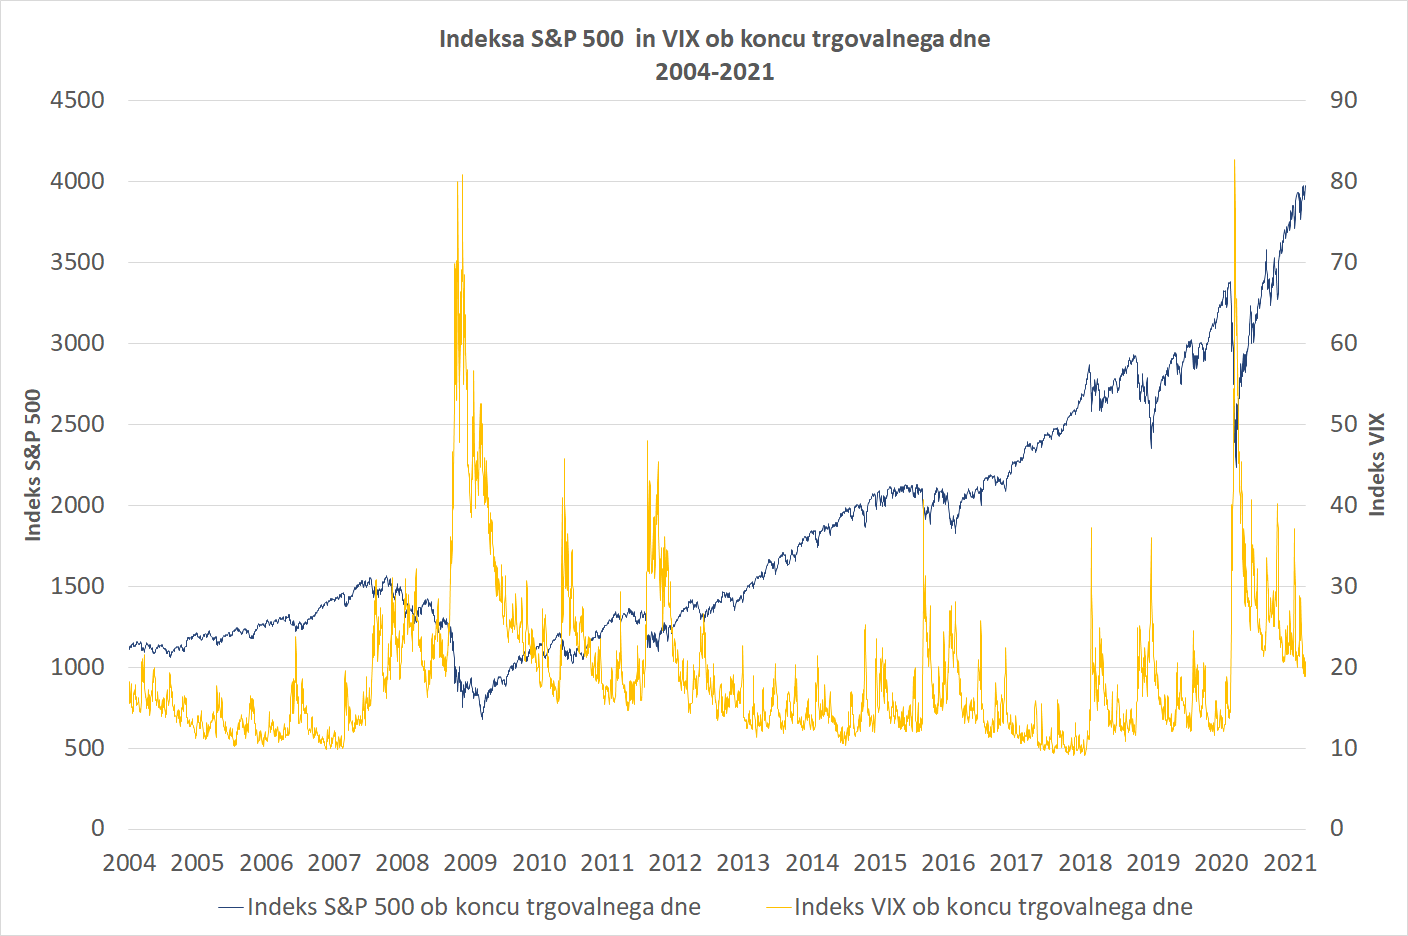
\includegraphics[width = 15 cm]{Grafi/VIX_vs_SPX_2004-2021.png}
\caption{Vrednosti indeksa VIX in S\&P~500 v obdobju 2004--2021, vir: Yahoo finance}
\label{Graf 2}
\end{figure}


Iz slike \ref{Graf 2} sta razvidni še dve lastnosti gibanja vrednosti indeksa VIX:
\begin{itemize}
\item Porazdelitve vrednosti indeksa VIX so asimetrične z daljšim repom v pozitivni smeri (angl. \textit{positively skewed}). Vrednost indeksa se redkeje poveča, a v teh primerih je rast vrednosti visoka, medtem ko je padanje vrednosti indeksa bolj pogosto, so pa dnevni padci manjši. Vrednosti indeksa se v času občasnih rasti povečujejo zelo hitro, nato pa dlje časa postopoma padajo.\\

\item Vrednosti indeksa VIX se po vsakem dvigu ali padcu normalizirajo. Pravimo, da vrednost indeksa teži k povprečju (angl. \textit{mean-reverting}).
\end{itemize}

\begin{figure}[!h]
\centering
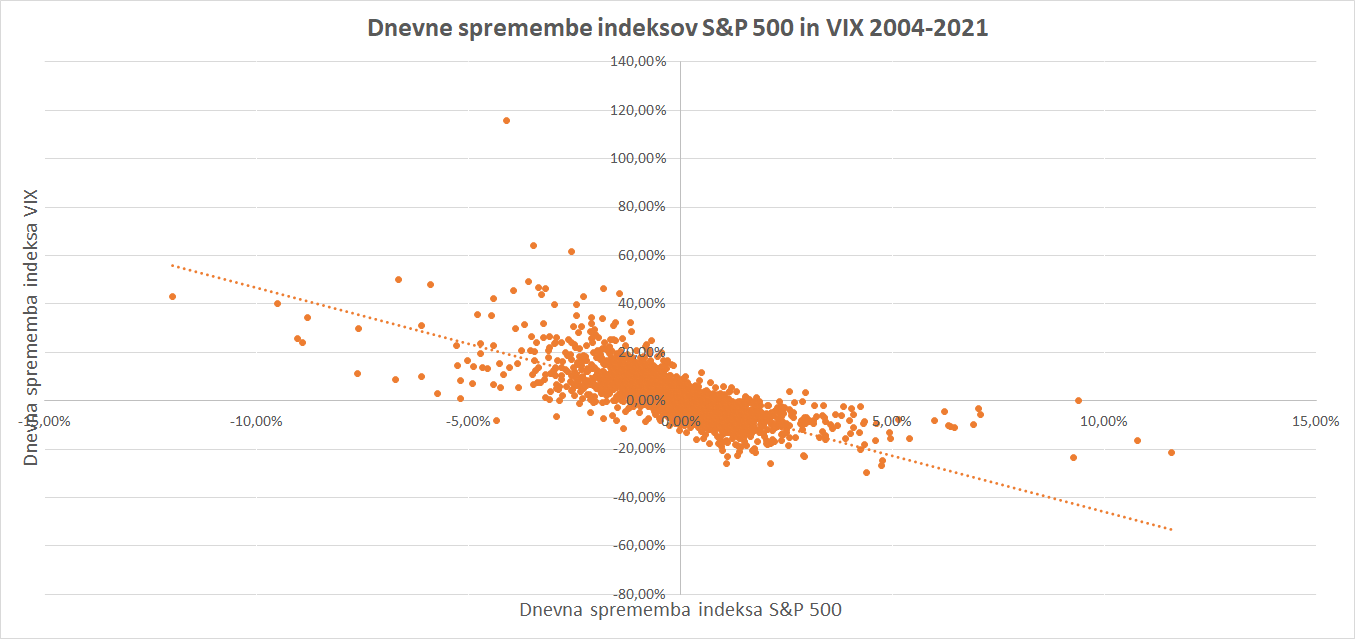
\includegraphics[width = 15 cm]{Grafi/VIX_SPX_correlation.png}
\caption{Razsevni diagram dnevnih sprememb indeksov S\&P~500 in VIX v obdobju 2004--2021, vir: Yahoo finance}
\label{Graf 3}
\end{figure}


Rhoads v knjigi \cite{rhoads} predlaga predlaga sledečo formulo za izračun predvidene 30-dnevne volatilnosti indeksa S\&P~500 glede na dnevno vrednost indeksa VIX:
\begin{equation}
\label{eqn:VIX_predict}
\Delta_\% I_{500} = \frac{I_\text{VIX}}{\sqrt{12}}\%
\end{equation}
Če trenutna vrednost indeksa VIX znaša 25, je pričakovana 30-dnevna volatilnost indeksa S\&P~500 enaka 7,21~\%. To pomeni, da vlagatelji pričakujejo, da bo donosnost indeksa S\&P~500 v naslednjem mesecu najverjetneje znašala med -7,21~\% in 7,21\%.\\

Z zbranimi podatki lahko preverimo navedeno uporabo indeksa VIX. Za vsak dan v obdobju 2004--2021 preberemo vrednost indeksa VIX in izračunamo donosnost indeksa S\&P~500 v naslednjem mesecu (za poenostavitev vzamemo 20 delovnih dni). Na sliki \ref{Graf 9} je prikazan razsevni grafikon dobljenih točk s premicama, ki določata mejo na osnovi enačbe \ref{eqn:VIX_predict}. Opazimo...

\begin{figure}[!h]
\centering
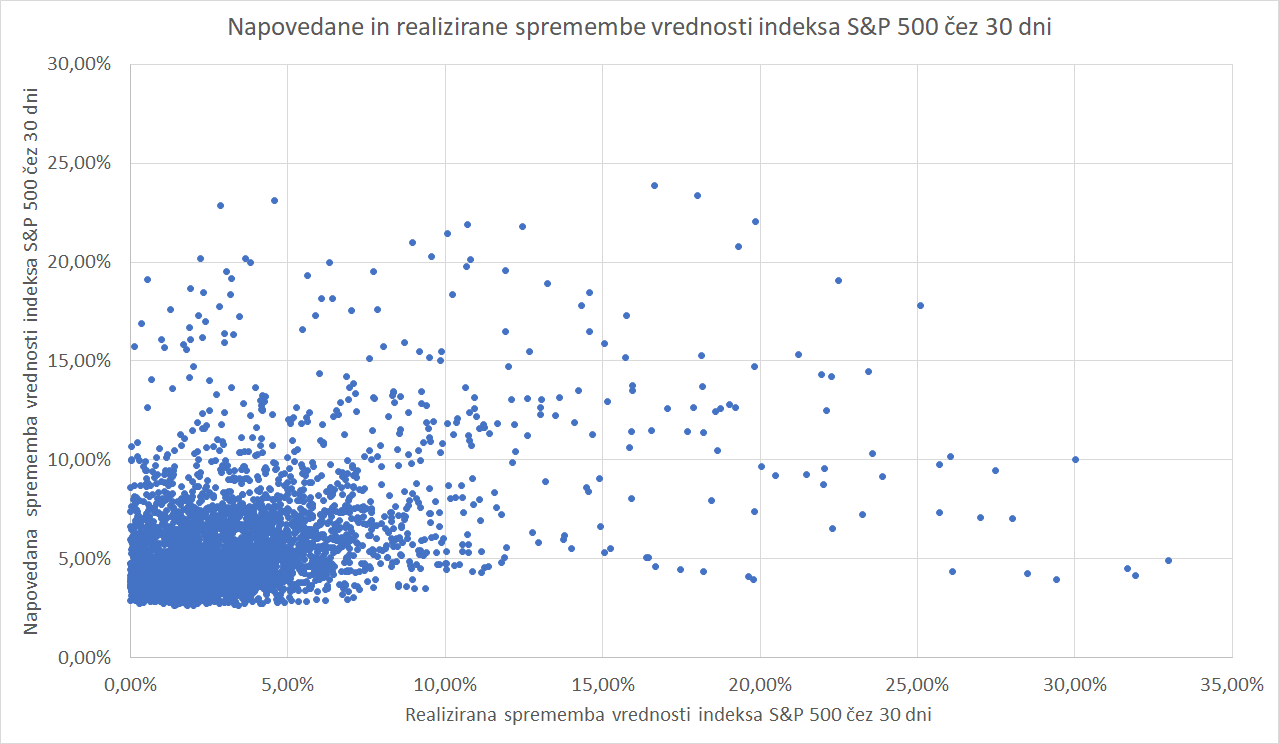
\includegraphics[width = 15 cm]{Grafi/SPX_prediction_with_VIX.png}
\caption{Razsevni diagram realiziranih in napovedanih 30-dnevnih sprememb indeksa S\&P 500 v obdobju 2004-2021}
\label{Graf 9}
\end{figure}




Vrednosti indeksa VIX v času rasti indeksa S\&P~500 (angl. \textit{bull market}) ostajajo nizke, saj vlagatelji ne bodo pretirano investirali v nakupne opcije na vrednost indeksa S\&P~500, ampak pogosteje v delnice ali investicijske sklade.\
V obdobju padanja vrednosti indeksa S\&P~500 (angl. \textit{bear market}) se močno poveča povpraševanje po prodajnih opcijah na indeks S\&P~500, posledično narastejo njihove premije in vrednost indeksa VIX se zviša.\\

Z vlaganjem v vrednosti indeksa VIX se lahko investitor zavaruje pred nenadnim padcem  vrednosti indeksa S\&P~500 in celotnega ameriškega in svetovnega gospodarstva, vendar direktne investicije v indeks VIX niso možne, saj je le indeks, izračunan s pomočjo opcij na vrednost indeksa S\&P 500, ki se ne splačajo. \\

Medtem ko je v praksi mogoče upravljati portfelj delnic, ki zelo natančno posnema donosnost indeksa S\&P 500 (nekateri investicijski skladi počnejo ravno to), je to za indeks VIX tudi v teoriji nemogoče.
Zato obstajajo različni finančni inštrumenti, katerih izplačila so odvisna od vrednosti indeksa VIX; to so terminske pogodbe na vrednost indeksa VIX in opcije na vrednost indeksa VIX, investitorji pa lahko tudi vlagajo v investicijske sklade volatilnosti (angl. \textit{volatility exchange-traded funds, volatility ETF}).



\section{Terminske pogodbe na vrednost indeksa VIX}
Terminske pogodbe na vrednost indeksa VIX (angl. \textit{VIX futures}) so bile prvič predstavljene leta 2004 in jih lahko najdemo pod oznako VX (mesečne terminske pogodbe) in VX01 do VX53 (tedenske terminske pogodbe).\

Mesečne terminske pogodbe imajo ročnost na sredo, ki je 30 dni pred petkom, ko zapadajo tradicionalne mesečne opcije na vrednost indeksa S\&P~500.
Terminske pogodbe na vrednost indeksa VIX so denarno poravnane z denarnim multiplikatorjem 1000 dolarjev.

Izročitvene vrednosti indeksa v terminskih pogodbah z bližanjem ročnosti konvergirajo k vrednosti VIX. Zaradi tega so kratkoročne terminske pogodbe veliko bolj občutljive na spremembe vrednosti indeksa VIX kot tiste z daljšo ročnostjo. Pogodbe z daljšo ročnostjo imajo običajno tudi višjo izročitveno vrednost kot pa tiste s krajšo ročnostjo. Stanju na trgu, ko so izročitvene vrednosti terminskih pogodb z daljšo ročnostjo višje od tistih s krajšo ročnostjo, imenujemo \textit{contango}. V nasprotnem primeru, ko so izročitvene vrednosti terminskih pogodb s krajšo ročnostjo višje od tistih z daljšo ročnostjo, tako stanje na trgu imenujemo \textit{backwardation}.\\

Na sliki \ref{Graf 6} so prikazane izročitvene vrednosti terminskih pogodb z različnimi ro\-čno\-stmi v obdobju med letoma 2017 in 2018. Opazimo, da so bile izročitvene vrednosti terminskih pogodb vse do februarja 2018 višje od trenutne vrednosti indeksa VIX, pri čemer višja izročitvena vrednost pripada pogodbi z daljšo ročnostjo. To je \textit{contango}. S padcem trga pa je vrednost indeksa VIX narasla in odnosi med trenutno in izročitvenimi vrednostmi indeksa VIX so prešli v \textit{backwardation}. Če primerjamo terminski pogodbi za februar in marec 2018, opazimo, da je bila izročitvena vrednost marčevske pogodbe do začetka februarja višja od februarske terminske pogodbe, po šoku na trgu pa je izročitvena vrednost februarske terminske pogodbe višja in je bila tudi bolj občutljiva na spremembe vrednosti indeksa VIX kot pa marčevska.
\begin{figure}[!h]
\centering
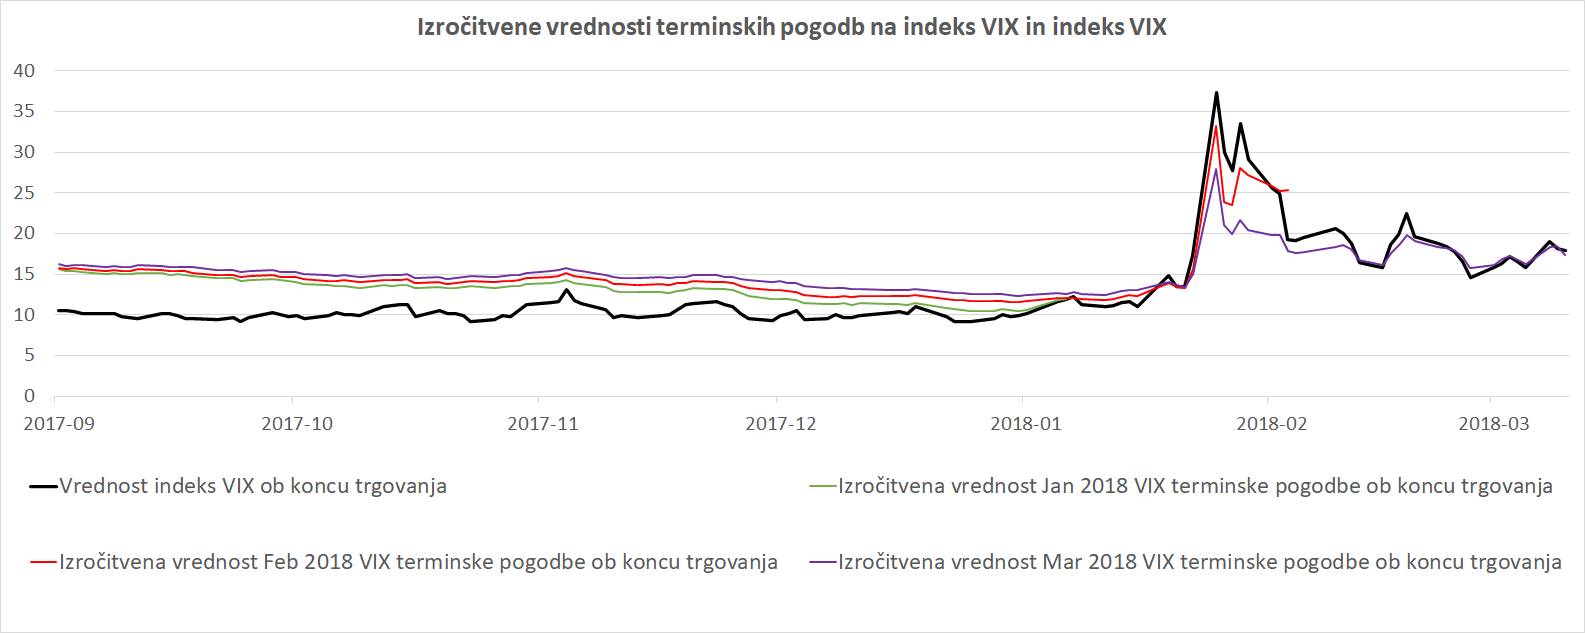
\includegraphics[width = 15 cm]{Grafi/VIX_futures_2018.png}
\caption{Gibanje izročitvenih vrednosti VIX mesečnih terminskih pogodb in vrednosti indeksa VIX, vir: CBOE}
\label{Graf 6}
\end{figure}\



Terminske pogodbe se ob ročnosti denarno poravnajo, vendar ne z vrednostjo indeksa VIX na dan poravnave temveč z vrednostjo njemu sorodnega indeksa volatilnosti za poravnave borze CBOE (angl. \textit{COBE Volatility index settlement}), za katerega se pogosto uporablja ime indeks VRO.\\

Medtem ko se za izračun indeksa VIX uporabijo opcije na vrednost indeksa S\&P~500, ki zapadejo čez več kot 23 in manj kot 37 dni, se za izračun vrednosti indeksa VRO uporabijo le opcije, ki zapadejo čez točno 30 dni. Indeksa VRO ni mogoče izračunati kadarkoli, ker morda ni opcij, ki zapadejo točno čez 30 dni. Datum poravnave terminskih pogodb je nastavljen tako, da tedaj indeks VRO lahko izračunamo.  Prav tako CBOE s svojim internim modelom določi interval izvršilnih vrednosti nakupnih in prodajnih opcij, ki bodo uporabljene v izračunu vrednost indeksa. Model za izbiro opcij, vključenih v izračun indeksa VRO, ni javno objavljen, na voljo je le seznam opcij, ki so bile uporabljene za izračun indeksa VRO. Čeprav se za izračun vrednosti indeks VIX ne uporabi opcij s ponujeno premijo 0, se pri izračunu vrednosti indeksa VRO takšne opcije lahko uporabijo.\\

Še ena razlika med izračunom vrednosti indeksa VIX in indeksa VRO je, da se za izračun indeksa VIX uporabi povprečje ponujene in povprašane premije posamezne opcije, medtem ko se za izračun vrednosti indeksa VRO uporabi vrednosti premij iz transkakcij ob začetku trgovalnega dne (angl. \textit{opening price}).\\

\textbf{Zgled.}
Oglejmo si primer poravnave mesečne terminske pogodbe na vrednost indeksa VIX. Vrednost indeksa VIX na dan 12. januar 2018 je bila 10,16, izročitvena vrednost februarske terminske pogodbe na vrednost VIX pa je bila 11,67.\
Če bi držali svojo pozicijo vse do ročnosti terminske pogodbe, bi se 14. februarja 2018, to je dan poravnave februarske terminske pogodbe na indeks VIX, terminska pogodba poravnala po vrednosti 21,87, kot je bila tisti dan vrednost indeksa VRO in ne po vrednosti indeksa VIX, ki je bila ob koncu trgovanja 19,26. Zaradi denarnega multiplikatorja 1\,000 dolarjev bi prodajalec teminske pogodbe moral plačati kupcu terminske pogodbe znesek:
$$
(21,\!87 - 11,\!67) \cdot 1\,000\,\$ = 10\,200\,\$.
$$

Običajno je situacija na delniškem trgu stabilna in posledično je vrednost indeksa VIX nizka in izročitvene vrednosti indeksa v  terminskih pogodbah so višje od trenutne vrednosti VIX. Če investitor meni, da bo prišlo do spremembe na trgu in s tem dviga vrednosti VIX, sklene dolgo pozicijo v terminski pogodbi. V primeru, da res pride do negotovosti na trgu in se vrednost indeksa VIX poveča, bo imel investitor dobiček, v nasprotnem primeru pa izgubo.\

V primeru, da je trg nestabilen in s tem vrednost indeksa VIX visoka, pa so izročitvene vrednosti indeksa v terminskih pogodbah nižje od vrednosti indeksa VIX.\

Zaradi razlik v izračunu vrednosti indeksov VIX in VRO se lahko na dan poravnave terminske pogodbe vrednosti indeksa VIX indeksa VRO razlikujeta, s tem pa tudi  izročitvena vrednost po kateri se poravna terminska pogodba.\\

Vrednosti  indeksov VIX in VRO za obdobje od leta 2013 do 2021 so prikazane na sliki \ref{Graf 7}. Vrednosti indeksov sta večino časa zelo blizu, z izjemo nekaterih krajših obdobij. Največja razlika je bila dosežena 14. decembra 2014, ko je bila vrednost indeksa VRO 24,09 in vrednost indeksa VIX 19,44.

\begin{figure}[!h]
\centering
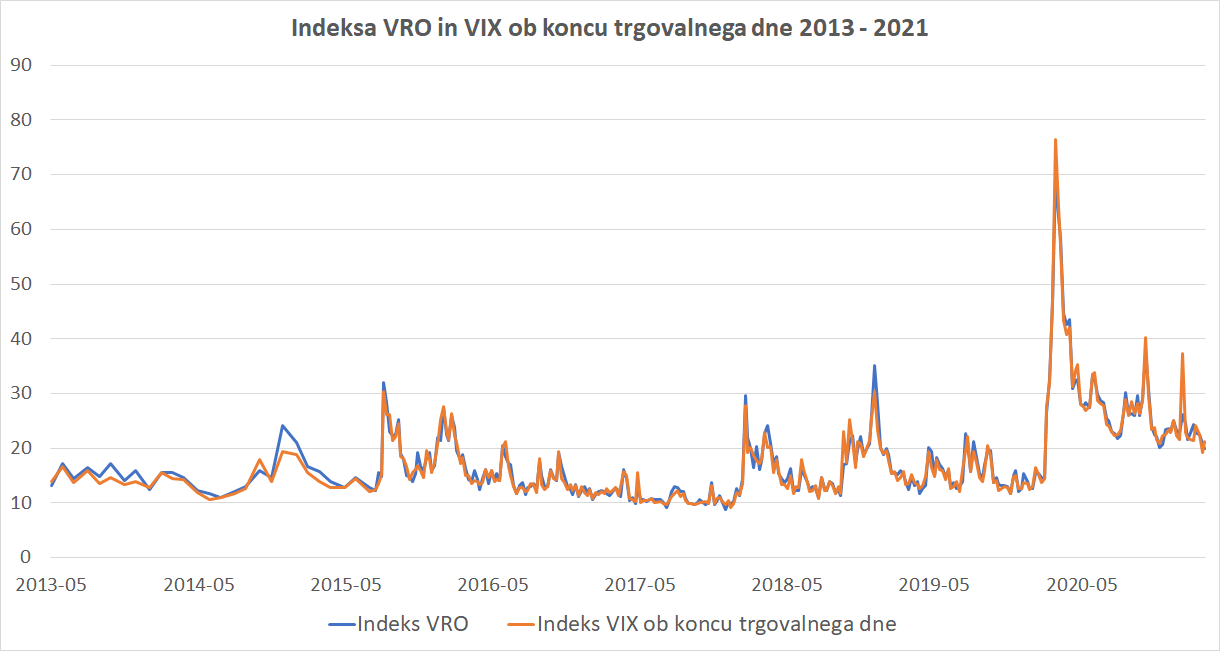
\includegraphics[width = 15 cm]{Grafi/VRO_VIX.png}
\caption{Gibanje vrednosti indeksov VRO in VIX v obdobju 2004--2021, vir: CBOE}
\label{Graf 7}
\end{figure}

Takšna dodatna negotovost za vlagatelja predstavlja dodaten riziko njegove investicije. Prav zaradi tega večina vlagateljev svoje terminske pogodbe na vrednost indeksa VIX dan pred ročnostjo proda in kupi terminske pogodbe s kasnejšim datumom ročnosti (angl. \textit{futures roll}).\

Ker so terminske pogodbe na VIX večino časa v \textit{contagu}, je vrednost terminske pogodbe s krajšo ročnostjo običajno nižja kot vrednost terminskih pogodb z daljšo ročnostjo. S tem ko vlagatelj dan pred ročnostjo terminske pogodbe naredi zamenjavo, s prodajo stare in nakupom nove terminske pogodbe utrpi dodaten strošek. Omenjen strošek se imenuje strošek držanja (angl. \textit{cost of carry}), in ga mora vlagatelj plačevati, če želi ohranjati svojo dolgo pozicijo v konstantnem številu terminskih pogodb. Zaradi dodatnega stroška ohranjanja pozicije je dolgoročno vlaganje v vrednost indeksa VIX neprofitabilno.\\

Neprofitabilnost dolgoročnega vlaganja v vrednost indeksa VIX ponazarja slika \ref{Graf 4}, na kateri je predstavljeno gibanje vrednosti portfeljev indeksa S\&P~500,  indeksa VIX in terminske pogodbe v letu 2019. Začetna vrednost vseh portfeljev je 100 dolarjev. Portfelja indeksov VIX in S\&P~500 sta teoretična, njuni vrednosti sta vsak dan določeni tako, da ohranjata sorazmerje z vrednostjo posameznega indeksa. Za vrednost portfelja iz terminskih pogodb na vrednost indeksa VIX privzamemo izročitvene vrednosti terminskih pogodb na indeks VIX s konstantnim datumom zapadlosti en mesec. Vsak dan s prodajo deleža VIX terminske pogodbe, ki zapade v najbližjem mesecu, in z nakupom deleža VIX terminske pogodbe, ki zapade en meseca kasneje, ohranjamo konstanten povprečen čas do ročnosti pogodb v portfelju. Količine prodanih in kupljenih pogodb določamo tako, da dobimo strategijo samofinanciranja.\

V letu 2019 ni bilo večjih pretresov na finančnih trgih. Če bi na začetku leta investirali 100 dolarjev v portfelj, ki sledi indeksu S\&P~500, bi ob koncu leta dosegli 28,7-odstotni dobiček. Z enako investicija v portfelj, ki sledi indeksu VIX, bi ob koncu leta dosegli 41-odstotno izgubo. Če bi na začetku leta investirali 100 dolarjev v portfelj terminskih pogodb, bi ob koncu leta dosegli 67-odstotno izgubo.
\begin{figure}[!h]
\centering
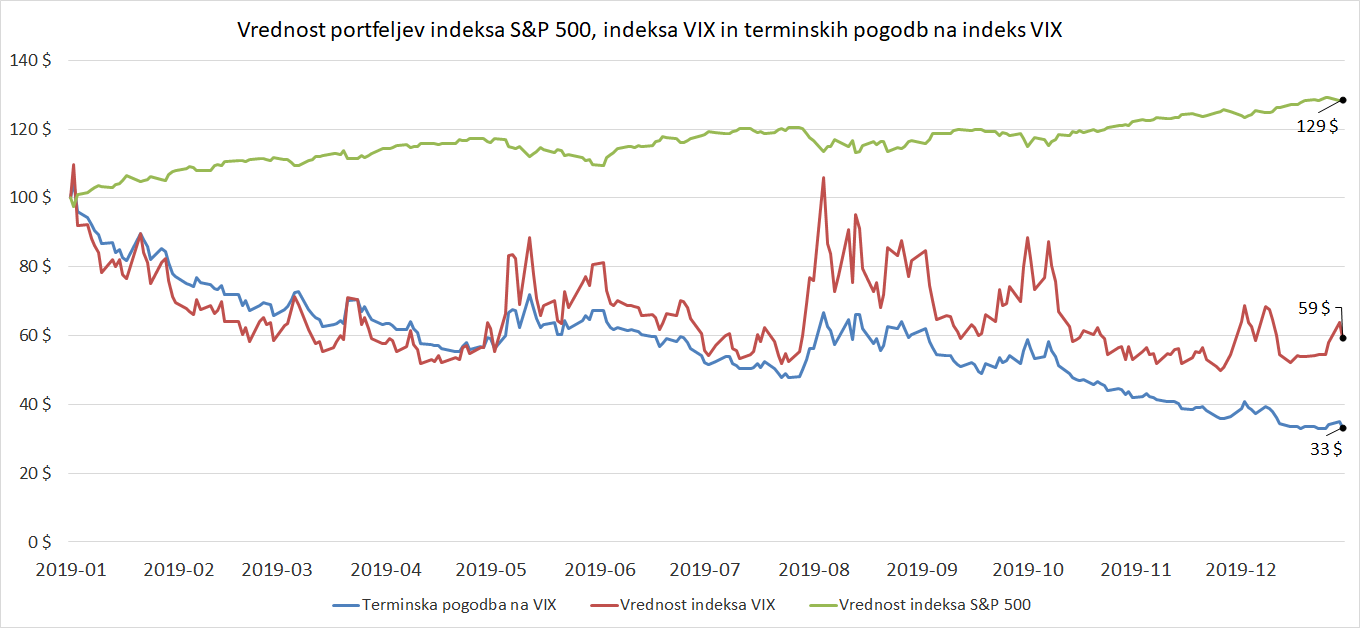
\includegraphics[width = 15 cm]{Grafi/Portfolio_VIX_futures_2019.png}
\caption{Gibanje vrednosti treh portfeljev z začetno vrednostjo 100 dolarjev v letu 2019, vir: S\&P Dow Jones Indices, Yahoo Finance}
\label{Graf 4}
\end{figure}

Slika \ref{Graf 5} prikazuje gibanje vrednosti treh takšnih portfeljev z začetno vrednostjo 100 dolarjev v letu 2020. Ob koncu leta bi realizirali 15-odstotno donosnost z investicijo v portfelj, ki sledi indeksu S\&P~500.  Z enako investicijo v portfelj, ki sledi indeksu VIX, bi ob koncu leta dosegli 82-odstotno donosnost. Če bi na začetku leta investirali 100 doalrjev v terminsko pogodbo, bi ob koncu leta dosegli 17-odstotni dobiček.\

Opazimo, da bi lahko investicija v portfelj, ki sledi indeksu VIX v sredini meseca marca, ko je indeks S\&P~500 padel za 31 odstotkov, realizirala 563-odstotni dobiček. Podobno bi investicija v portfelj terminskih pogodb na VIX v mesecu marcu realizirala 381-odstotni dobiček.\

Dogajanje v letu 2020 je zelo nazoren primer, kako bi lahko z investicijo v finančni inštrument, katerega vrednost je odvisna od vrednost indeksa VIX, zaščitili vrednost svojega portfelja, ki je odvisen od vrednosti indeksa S\&P~500.\

Investitor sam določi, kolikšen del sredstev bo vložil v posamezno vrsto portfelja. Ker v daljšem obdobju vrednost indeksa S\&P~500 pogosteje narašča kot pada, investicija enakih zneskov v terminske pogodbe na vrednost indeksa VIX in v indeks S\&P 500 pogosto ni najbolj učinkovita. Veliko bolj smiselna bi bila le 10 odstotna alokacija vrednosti investicije v terminsko pogodbo. Vijolična krivulja na sliki \ref{Graf 5} prikazuje gibanje vrednosti portfelja, v katerem smo na začetku leta 90 dolarjev investirali tako, da sledijo indeksu S\&P~500, 10 dolarjev pa terminske pogodbe na indeks VIX. Opazimo, da donos, ki ga ustvarja del portfelja, investiran v indeks S\&P~500, nadomesti stroške investicije v terminske pogodbe na indeks VIX. S tem ustvarimo portfelj, katerega vrednost počasi raste tudi preko zelo turbolentnih obdobji.

\begin{figure}[!h]
\centering
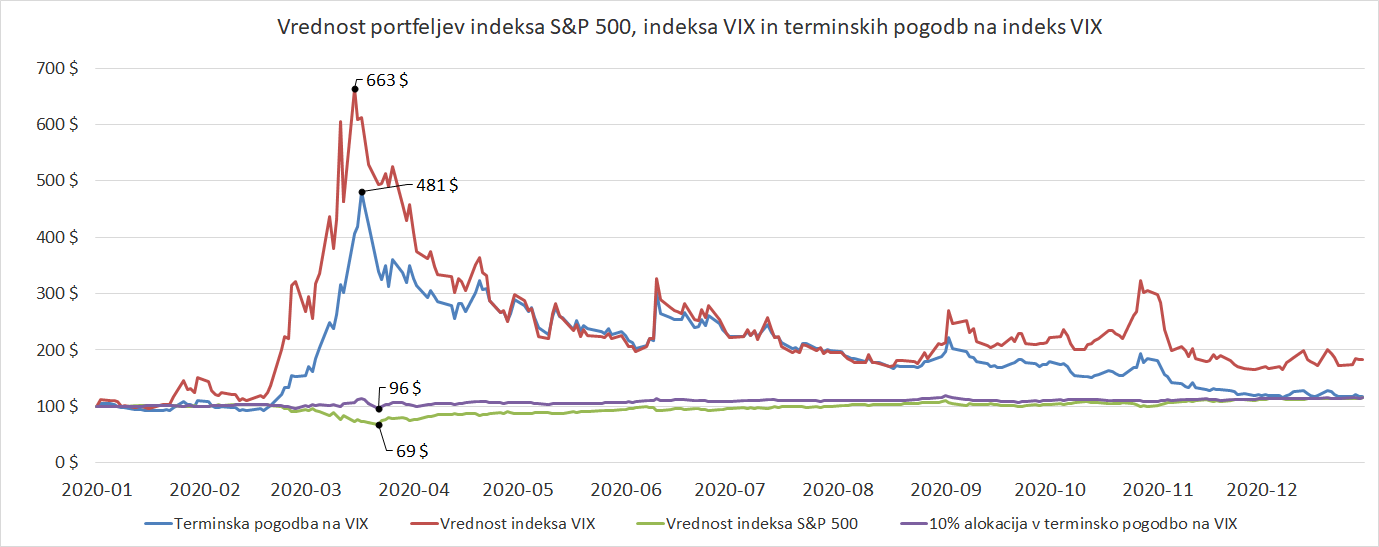
\includegraphics[width = 15 cm]{Grafi/Portfolio_VIX_futures_2020.png}
\caption{Gibanje vrednosti portfeljev z začetno vrednostjo 100 dolarjev v letu 2020, vir: S\&P Dow Jones Indices, Yahoo Finance}
\label{Graf 5}
\end{figure}

Terminske pogodbe na indeks VIX (in v nadaljevanju tudi opcije na VIX) so namenjene ščitenju (angl. \textit{hedge}) portfelja, saj ob šoku na finančnem trgu ustvarijo donos, ki nadomesti padec vrednosti portfelja. Ker mora investitor ob dvigu vrednosti finančnih inštrumentov na indeks VIX svojo pozicijo zapreti, omenjeni finančni instrumenti niso primerni za pasivnega investitorja.

\section{Opcije na vrednost indeksa VIX}
Opcije na vrednost indeksa VIX (angl. \textit{VIX options}) so bile prvič na voljo leta 2006 in jih najdemo pod kratico VIX. Opcije so evropske in imajo podobno kot terminske pogodbe na indeks VIX zapadlost na sredo, ki je 30 dni pred petkom, ko zapadejo tradicionalne mesečne opcije na vrednost indeksa S\&P~500, in so denarno poravnane.\
Medtem ko je denarni multiplikator za terminsko pogodbo 1\,000 dolarjev, je denarni multiplikator pri opcijah na indeks VIX 100 dolarjev.
LetA 2009 so bile na trgu prvič ponujene tudi tedenske VIX opcije. Uveljavila sta se izraza VIX opcije za prvotne, mesečne opcije na vrednost indeksa VIX in VIX tedenske opcije za tedenske opcije na vrednost indeksa VIX.\\

Medtem ko so vrednosti terminskih pogodb na indeks VIX neposredno vezane na vrednost indeksa VIX, pa so opcije na indeks VIX vezane na vrednost VIX terminske pogodbe z enako ročnostjo (oziroma indeks VRO). Kot hipotetični primer se lahko zgodi, da je vrednost indeksa VIX 30, medtem ko je ponujena premija nakupne opcije z izvršilno vrednostjo 25 in z zapadlostjo čez en mesec nizka. Na prvi pogled se zdi, da se bo opcija ob zapadlosti splačala, vendar mora investitor pregledati izročitveno vrednost terminske pogodbe na VIX z enakim datumom ročnosti, kot ga ima opcija. Ker je povprašana premija nakupne opcije nizka, trg verjetno pričakuje, da bo vrednost indeksa VIX ob času zapadlosti opcije nižja kot 25, pričakovano vrednost indeksa VIX pa izraža izročitvena vrednost terminske pogodbe na indeks VIX.\
Podobno kot pri terminskih pogodbah se z sklenitvijo nakupne VIX opcije zavarujemo pred šokom na finančnem trgu.\\

Na sliki \ref{Graf 8} so predstavljeni povprečni dnevni obsegi trgovanja z opcijami na vrednost indeksa VIX po mesecih za obdobje od leta 2007 do leta 2021.\
Ker so bile VIX opcije prvič na voljo šele leta 2006, jih v času finančne krize v letu 2008 niso uporabljali v večjem obsegu. Obseg trgovanja z VIX opcijami se je v naslednjih letih povečeval in dosegel svoj vrh v času povišane volatilnosti na trgu februarja 2018.

Po rekordnem obsegu v februarju 2018 je obseg trgovanja z VIX opcijami upadel in ostal nizek vse do marca leta 2020, ko se je interes vlagateljev po VIX opcijah zaradi negotovosti ob začetku epidemije covida-19 spet povečal.

\begin{figure}[!h]
\centering
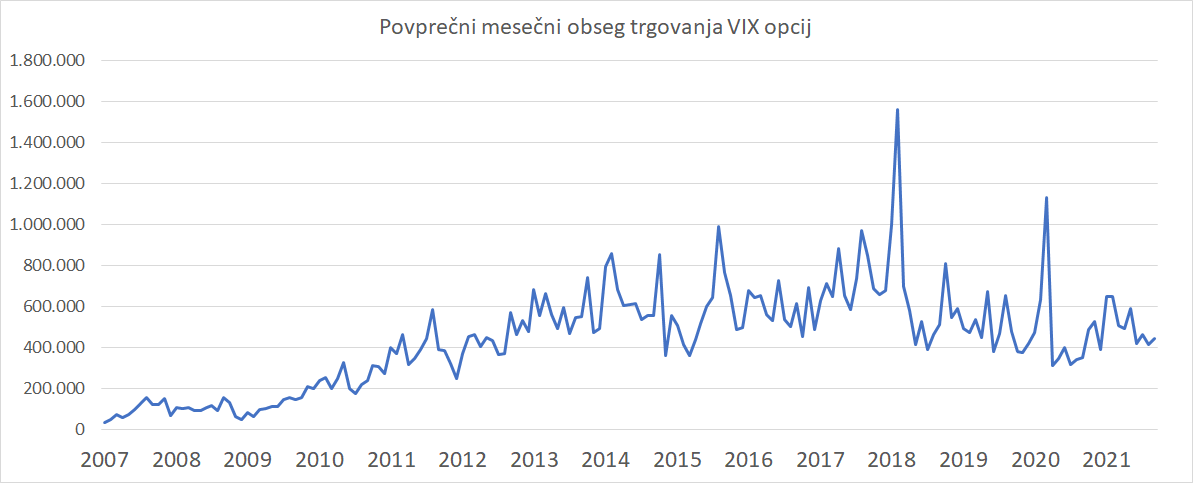
\includegraphics[width = 15 cm]{Grafi/VIX_options_volume.png}
\caption{Povprečni dnevni obseg trgovanja VIX opcij po mesecih v obdobjih 2007--2021, vir: CBOE}
\label{Graf 8}
\end{figure}


Na sliki \ref{Graf 10} je predstavljeno gibanje vrednosti indeksa VIX in ponujenih premij nakupnih opcij na VIX z izvršilno vrednostjo 20. Za prikaz je bila izbrana izvršilna vrednost 20, saj imajo nakupne opcije tudi v času nizke volatilnosti indeksa S\&P~500 nezanemarljivo povprašano premijo.\
Opazimo, da imajo nakupne opcije na vrednost indeksa VIX z daljšim časom do zapadlosti v obdobju brez šoka na finančnem trgu višjo ponujeno premijo kot pa tiste s krajšo ročnostjo. Ob trenutnku, ko se šok zgodi, se ponujene premije nakupnih opcij na vrednost indeksa VIX s krajšo zapadlostjo povečajo bolj kot pa tiste z daljšo zapadlostjo. Gibanje ponujenih premij nakupnih opcij na indeks VIX je zelo podobno gibanju izvršilnih vrednosti terminskih pogodb na indeks VIX z enako ročnostjo. \newline

\begin{figure}[!h]
\centering
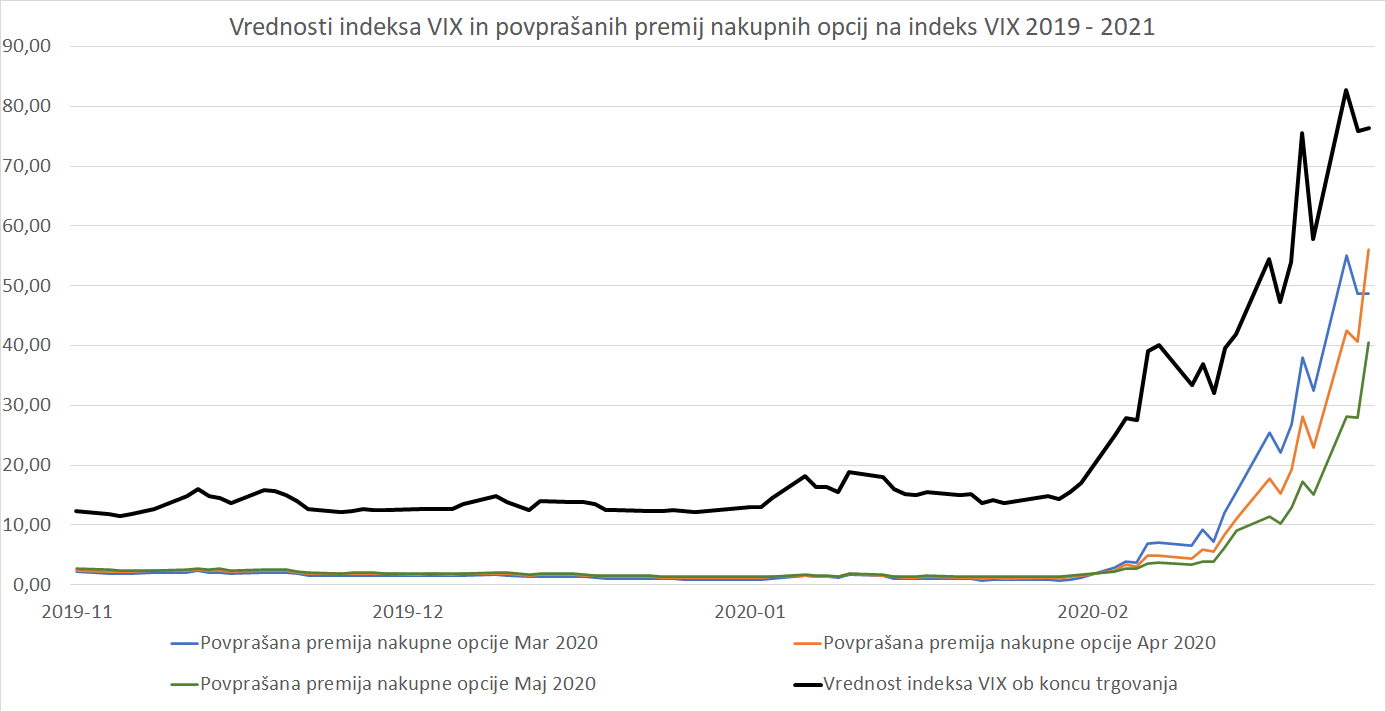
\includegraphics[width = 15 cm]{Grafi/VIX_call_options_20.png}
\caption{Gibanje vrednosti indeksa VIX in povprašanih premij nakupnih opcij na VIX v obdobju 2019--2020, vir: Barchart}
\label{Graf 10}
\end{figure}

\textbf{Zgled.}
Oglejmo si primer poravnave mesečne nakupne opcije na vrednost indeksa VIX.  Vrednost indeksa VIX na dan 17. januar 2020 je bila 12,10 in ponujena premija za marčevsko nakupno opcijo z izvršilno vrednostjo 20 je znašala 0,9.\
Zaradi denarnega multiplikatorja 100 dolarjev za nakup nakupne opcije plačamo $100\,\$ \cdot 0,\!90 = 90\,\$$.\
Če bi držali svojo pozicijo vse do zapadlosti opcije, bi se 18. marca 2020, na dan poravnave marčevskih opcij na indeks VIX, opcija poravnala po vrednosti 69,76 in ne po vrednosti indeksa VIX, ki je ob koncu trgovanja znašala 76,45. S tem bi bilo izplačilo nakupne opcije:
$$
(69,\!76 - 20) \cdot 100\,\$ = 4\,976\,\$,
$$
donos investicije (če zanemarimo časovno vrednost denarja) pa:
$$
4\,976\,\$ -90\,\$ = 4\,886\,\$.
$$
Čeprav je vrednost indeksa S\&P~500 leta 2020 v času negotovosti ob izbruhu svetovne epidemije covida-19, znižala za 33~\%, bi z nakupom nakupne opcije na indeks VIX le dva meseca prej dosegli skoraj 543~\% donosnost.




%\section*{Slovar strokovnih izrazov}

% slovar
%\geslo{}{}
%
%\geslo{}{}
%

\newpage
\begin{thebibliography}{99}

\bibitem{}
E.~Szado, \emph{Selling VIX futures and options for portfolio enchancement}, Working paper, CBOE, Chicago, 2019.

\bibitem{}
E.~Szado, \emph{The portfolio diversification potential of long VIX futures and options strategies}, Working paper, CBOE, Chicago, 2019.

\bibitem{}
E.~Szado, \emph{VIX futures and options -- A case study of portfolio diversification during the 2008 financial crisis}, Working paper, CBOE, Chicago, 2009.

\bibitem{rhoads}
R.~Rhoads, \emph{Trading VIX derivatives: Trading and hedging strategies using VIX futures, options, and exchange-traded notes}, John Wiley \& Sons, New Jersey, 2011.

\bibitem{whaley}
R.~Whaley, \emph{Understanding the VIX}, The Journal of Portfolio Managment \textbf{35} (2009), 4--5.

\bibitem{morgan_stanley}
Morgan Stanley's Institutional Equity Division Sales Desk, \emph{A guide to VIX futures and options}, QDS Vega Times, Morgan Stanley, 2011.

\bibitem{hedging_spx_vix}
B.~Lerner in C.~Metli, \emph{The art of hedging}, Risk Managment Newsletter \textbf{33}, 2015.

\bibitem{}
\emph{VIX white paper}, v: CBOE, [ogled 17. 11. 2019], dostopno na \url{https://cdn.cboe.com/resources/vix/vixwhite.pdf}.

\bibitem{}
\emph{Vrednost indeksa S\&P~500}, v: Yahoo finance, [ogled 31. 3. 2021], dostopno na \url{https://finance.yahoo.com/quote/%5EGSPC/history?p=%5EGSPC}.

\bibitem{}
\emph{Vrednost indeksa VIX}, v: Yahoo finance, [ogled 31. 3. 2021], dostopno na \url{https://finance.yahoo.com/quote/%5EVIX/history?p=%5EVIX}.

\bibitem{}
\emph{Vrednost indeksa VRO}, v: CBOE, [ogled 26. 8. 2021], dostopno na \url{https://www.cboe.com/us/futures/market_statistics/final_settlement_prices/}.

\bibitem{spx_companies}
\emph{Tržni deleži podjetij v indeksu S\&P~500}, v: Slickcharts, [ogled 4. 9. 2021], dostopno na \url{https://www.slickcharts.com/sp500}.

\bibitem{apple_capitalization}
\emph{Prosta tržna kapitalizacija podjetja Apple}, v: GuruFinance, [ogled 15. 8. 2021], dostopno na \url{https://www.gurufocus.com/term/FloatPercentageOfTSO/aapl/Float-Percentage-Of-Total-Shares-Outstanding/Apple}.

\bibitem{spx_devisor}
\emph{Vrednost indeksnega delitelja indeksa S\&P~500}, v: ycharts, [ogled 15. 8. 2021], dostopno na \url{https://ycharts.com/indicators/sp_500_divisor}.

\bibitem{spx_cap}
\emph{Vrednost finančnih inštrumentov, odvisnih od vrednosti indeksa S\&P~500}, v: S\&P Global, [ogled 24. 8. 2021], dostopno na \url{https://www.spglobal.com/spdji/en/indices/equity/sp-500/#overview}.

\bibitem{}
\emph{Izročitvene vrednosti terminskih pogodb na indeks VIX}, v: CBOE, [ogled 17. 11. 2019], dostopno na \url{https://www.cboe.com/us/futures/market_statistics/historical_data/}.

\bibitem{}
\emph{Izročitvena vrednost terminske pogodbe na indeks VIX s konstantnim datumom zapadlosti 1 mesec}, v: S\&P Dow Jones Indices, [ogled 23. 8. 2021], dostopno na \url{https://www.spglobal.com/spdji/en/indices/strategy/sp-500-vix-short-term-index-mcap/#overview}.

\bibitem{}
\emph{Dnevni obseg trgovanja opcij na indeks VIX}, v: CBOE, [ogled 26. 8. 2021], dostopno na \url{https://www.cboe.com/us/options/market_statistics/historical_data/}.











\end{thebibliography}

\end{document}

